The following circuit is contructed for dc analysis.

\FloatBarrier

\begin{figure}[h!]
	\centering
	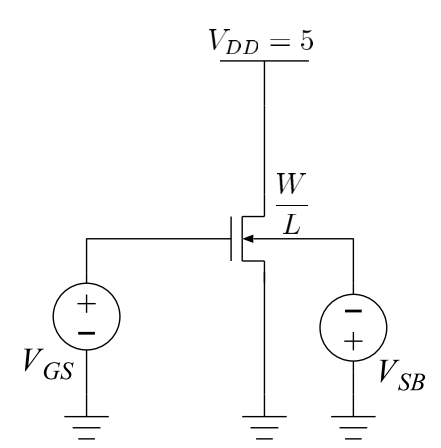
\includegraphics[scale=0.75]{../images/circuit_1.PNG}
	\caption{Circuit 1}
	\label{fig:circuit_1}
\end{figure}

\FloatBarrier

$V_{GS}$ is swept from $0$ \si{\volt} to $5$ \si{\volt} in increments of $0.2$ \si{\volt} and $i_D$ is measured at each value of $V_{GS}$. 
The results are plotted and tabulated below.

\FloatBarrier

\begin{figure}[h!]
	\centering
	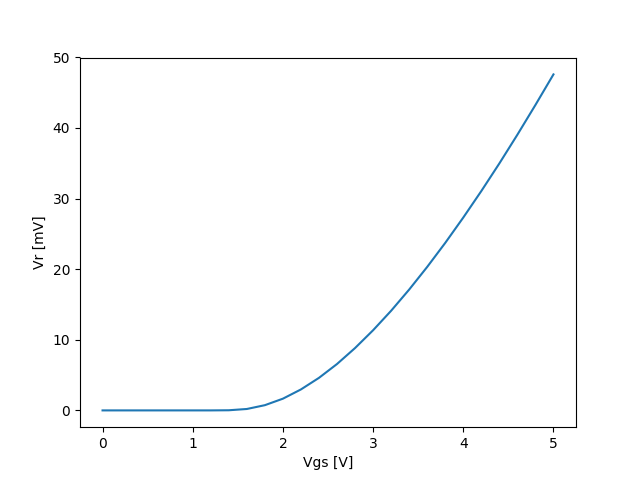
\includegraphics[scale=0.75]{../images/data_1.PNG}
	\caption{$i_{D}$ versus $V_{GS}$ of NMOS where $V_{SB}= 0$\si{\volt}}
	\label{fig:data_1}
\end{figure}

\FloatBarrier

\begin{table}[h!]
	\centering
	\caption{Figure (\ref{fig:data_1}) Data}
	\label{tab:data_1}
	\csvautotabular{../tables/data_1.csv}
\end{table}

\FloatBarrier

When a gate voltage $V_{GS}$ is applied to the NMOS, an electric field is generated across the metal gate and p-type substrate. 
This electric field repels majority holes from the surface of the substrate, creating a depletion region. 
The NMOS operates in cutoff region for $V_{GS}$ between $0$ \si{\volt} to about $1.5$ \si{\volt}. \\

When $V_{GS}$ exceeds $1.5$ \si{\volt}, donor electrons move to the surface of the substrate to form an n-type channel between the drain and source of the NMOS. 
This voltage is the threshold voltage $V_{tn}$. 
At this point, the NMOS is operating in saturation region because the saturation condition, $V_{DS} > V_{GS} - V_{tn}$ is met.
This is clear, as $V_{DS} = V_D - V_S = V_{DD} - 0 = 5$ \si{\volt} and $V_{GS}$ never exceeds $5$ \si{\volt}.
In saturation mode, the drain current is observed to quadratically increase as the gate voltage increases.
This is consistant with the drain current equation for NMOS in saturation, $i_D = \frac{1}{2}k_n' \frac{W}{L} (V_{GS} - V_{tn})^2$. \\

Then, $V_{SB}$ is set to $5$ \si{\volt} so a negative voltage is applied to the bulk of the NMOS, and the experiment is repeated.
The results are plotted and tabulated below. \\

\FloatBarrier

\begin{figure}[h!]
	\centering
	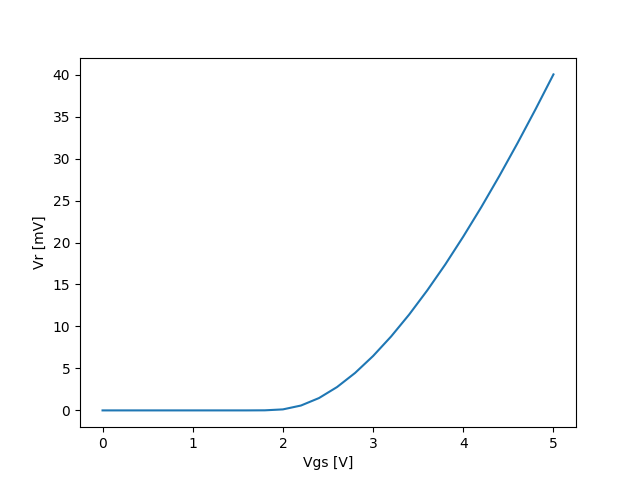
\includegraphics[scale=0.75]{../images/data_1_lower_body.PNG}
	\caption{$i_{D}$ versus $V_{GS}$ of NMOS where $V_{SB}= 0.5$\si{\volt}}
	\label{fig:data_1_b}
\end{figure}

\FloatBarrier

\begin{table}[h!]
	\centering
	\caption{Figure (\ref{fig:data_1_b}) Data}
	\label{tab:data_1_b}
	\csvautotabular{../tables/data_1_lower_body.csv}
\end{table}

\FloatBarrier

The negative voltage applied to the bulk of the NMOS causes the depletion region between the heavily doped n-type drain/source and the p-type substrate to widen. 
The wider depletion region impedes the formation of the n-type channel and the gate voltage must be increased to compensate.
This effectively increases the threshold voltage of the NMOS.
This also agrees with the Shichman-Hodges model for the body effect of MOSFETs, $V_{tn} = V_{to} + \gamma(\sqrt{2\phi_f + V_{SB}} - \sqrt{2\phi_f})$ where $V_{to}$ is the threshold voltage when no voltage is applied to the body, $\gamma$ is the body effect parameter and $\phi_f$ is the bulk potential of the MOSFET.
In this experiment, the threshold voltage $V_{tn}$ increased from $1.5$ \si{\volt} to about $1.9$ \si{\volt}.

Refer to Part 3 for $\frac{W}{L}$ ratio of the NMOS.